% ============================================================
%  第九章
% ============================================================
\section{合流：$\RR\times C$ 上的 Bogomolny 方程}
\markboth{第九章\ 合流：$\RR\times C$ 上的 Bogomolny 方程}{第九章\ 合流：$\RR\times C$ 上的 Bogomolny 方程}

\noindent{\small\color{shuyiGray}对应底本：原 p.49--p.54。}\par\medskip

\subsection{从线算子到 Bogomolny 方程}

\srcp{49}但这和几何 Hecke 变换有什么关系呢？这里我们得考虑 Bogomolny 方程，粗略地说，因为它们在四维超对称规范理论里支配一个\emph{时间无关}的情形。正如我们先前讨论过的，Bogomolny 方程是在三维的；而在三维里，余维 $3$ 的奇点是一个孤立点。

\begin{figure}[htbp]
\centering
\begin{tikzpicture}[scale=1.0]
  \draw[thick] (0,0) -- (1.7,0) -- (1.7,1.5) -- (0,1.5) -- cycle;
  \draw[thick] (0.45,0.4) -- (2.15,0.4) -- (2.15,1.9) -- (0.45,1.9) -- cycle;
  \draw[thick] (0,0) -- (0.45,0.4);
  \draw[thick] (1.7,0) -- (2.15,0.4);
  \draw[thick] (0,1.5) -- (0.45,1.9);
  \draw[thick] (1.7,1.5) -- (2.15,1.9);
  \fill[red!70!black] (1.05,0.92) circle (2.2pt);
  \draw[->,gray] (1.15,1.0) -- (1.5,1.5);
  \node[right,gray] at (1.5,1.55) {\scriptsize 孤立奇点};
  \node at (1.05,2.1) {\small $\RR^3$};
\end{tikzpicture}
\caption{三维中一个余维 $3$ 的奇点就是一点。't Hooft 算子的奇点，在 $\RR^3$ 里正是单极子的位置。}
\label{fig:codim3}
\end{figure}

所以我们得求解带有狄拉克单极子型孤立奇点的 Bogomolny 方程。（带这类奇点的 Bogomolny 方程，最早由 Kronheimer 在 1986 年研究，随后是 Pauly 在 1990 年。）

\subsection{$\RR\times C$：把 $\RR^3$ 换成“一族 Riemann 面”}

\srcp{50}在描述支配 $\RR^3$ 上 Bogomolny 方程解的“谱曲线”时，Atiyah 与 Hitchin 用了分解 $\RR^3=\RR\times\RR^2$，把 $\RR^3$ 看成 $\RR$ 的两参数族。这里我们改用同一个分解，但把 $\RR^3$ 看成 $\RR^2$ 的一参数族。其实，我们可以把 $\RR^2$ 换成任何 Riemann 面 $C$。于是我们将研究 $\RR\times C$ 上的 Bogomolny 方程，把它看成 $C$ 的一参数族。图像是这样的，其中用实变量 $y$ 参数化 $\RR$：

\begin{figure}[htbp]
\centering
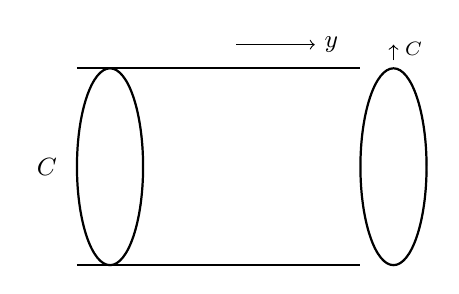
\begin{tikzpicture}[scale=1.0]
  \draw[thick] (0,0) ellipse (0.42 and 1.25);
  \draw[thick] (3.6,0) ellipse (0.42 and 1.25);
  \draw[thick] (-0.42,1.25) -- (3.18,1.25);
  \draw[thick] (-0.42,-1.25) -- (3.18,-1.25);
  \draw[densely dashed] (0,-1.25) arc (-90:90:0.42 and 1.25);
  \draw[densely dashed] (3.6,-1.25) arc (-90:90:0.42 and 1.25);
  \node[left] at (-0.55,0) {\small $C$};
  \draw[->] (1.6,1.55) -- (2.6,1.55) node[right] {\small $y$};
  
  \draw[->] (3.6,1.35) -- (3.6,1.55);
  \node[right] at (3.62,1.5) {\scriptsize $C$};
\end{tikzpicture}
\caption{$\RR\times C$ 看成 $C$ 的一参数族：轴向是 $\RR$，每个横截面都是同一条 Riemann 面 $C$。}
\label{fig:cylinder}
\end{figure}

\subsection{Atiyah--Bott：全纯结构与 $y$ 无关}

\srcp{51}正如 Atiyah 与 Bott 所解释的，$G$-丛 $E\to C$ 上的任何联络 $A$（$C$ 是 Riemann 面）都决定一个全纯 $G_\CC$-丛 $E_\CC$：只需取 $A$ 的 $(0,1)$ 部分，用它来定义 $E$ 的复化上的全纯结构。因此，$C\times\RR$ 上的任何规范场 $A$ 都决定一族全纯丛 $E_y\to C$，$y\in\RR$。不过，如果 $A$ 满足 Bogomolny 方程
\[
  F=\star\,\dd_A\phi
\]
（对某个 $\phi$），那么 $E_y$ 作为 $C$ 上的全纯丛，就\emph{典范地}与 $y$ 无关。这是对的，因为 Bogomolny 方程的 $3$ 个实分量中有 $2$ 个可以写成
\begin{equation}
  0=\Bigl[\frac{D}{Dy}+\ii\phi,\ \frac{D}{D\bar z}\Bigr].
  \label{eq:indep}
\end{equation}
这个条件告诉我们：要证明 $E_y$ 的复结构与 $y$ 无关，需要作怎样的规范变换。（第三个 Bogomolny 方程可以看成一个矩映射条件，这与 Atiyah 和 Bott 在讨论二维杨--米尔斯理论时所说的类似。）

\subsection{跨过 $y_0$：Hecke 修改}

\srcp{52}现在假设在某个点 $p\times y_0\in C\times\RR$ 处有一个 't Hooft/狄拉克奇点：

\begin{figure}[htbp]
\centering
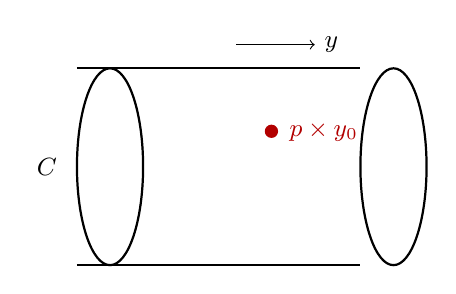
\begin{tikzpicture}[scale=1.0]
  \draw[thick] (0,0) ellipse (0.42 and 1.25);
  \draw[thick] (3.6,0) ellipse (0.42 and 1.25);
  \draw[thick] (-0.42,1.25) -- (3.18,1.25);
  \draw[thick] (-0.42,-1.25) -- (3.18,-1.25);
  \draw[densely dashed] (0,-1.25) arc (-90:90:0.42 and 1.25);
  \node[left] at (-0.55,0) {\small $C$};
  \fill[red!70!black] (2.05,0.45) circle (2.4pt);
  \node[right=3pt,red!70!black] at (2.05,0.45) {\small $p\times y_0$};
  \draw[->] (1.6,1.55) -- (2.6,1.55) node[right] {\small $y$};
\end{tikzpicture}
\caption{在 $\RR\times C$ 的 $(p,y_0)$ 处放一个 't Hooft/狄拉克奇点。$y$ 方向的切片 $E_y$ 在 $y\ne y_0$ 时彼此典范同构；只有在 $y=y_0$ 处，它才在 $p$ 点被“拧”了一下。}
\label{fig:hecke2}
\end{figure}

那么 $E_y$ 除 $y=y_0$ 外仍然典范地与 $y$ 无关。而且，即使跨过 $y=y_0$，只要把 $E_y$ 限制到 $C\setminus p$ 上，它仍然典范地与 $y$ 无关。换句话说，在 $y=y_0$ 处发生的事情是：丛 $E_y$ 在点 $p$ 作了一次 \emph{Hecke 修改}。Hecke 修改的“型”由那个特定的 't Hooft/狄拉克奇点决定，而它联系着 $\rho:U(1)\to T$。电—磁对偶把它联系到某个 $\rho^\vee:\Tvee\to U(1)$，从而联系到对偶群的表示。几何 Hecke 修改与对偶群表示之间的这个关系，正是几何 Langlands 对应所断言的那个关系。

\subsection{两个模空间重合}

\srcp{53}Bogomolny 方程解的模空间，与代数几何里定义的 Hecke 修改的模空间是重合的；这一点可以从“第三个” Bogomolny 方程的“矩映射”解释得出。

\subsection{收束}

\srcp{54}简而言之，我解释了规范理论对几何 Langlands 对应的解释里的某些主要想法。我试着描述了这个故事如何从 1970 年代 Goddard、Nuyts、Olive 的工作，以及随后 Montonen 与 Olive 的工作开始；我说了说这个故事如何与数学、物理中的其他发展并行展开；我也解释了 Michael Atiyah 在这一过程中所起的影响。

\begin{pizhu}{为什么 Bogomolny 方程是“时间无关”的四维方程}
四维超对称规范理论里有这样一个约化：取场不依赖时间 $t$，并要求 $A_t=\phi$、$F_{0i}=D_i\phi$。这正是 Bogomolny 方程 $F=\star\dd_A\phi$ 的“自对偶”部分；剩下的分量给出 $\dd_A\star F$ 之类的方程。在这种约化下，四维的 BPS 方程恰好变成三维的 Bogomolny 方程，而能量变成三维的能量泛函。

Witten 说“粗略地说，因为它们在四维超对称规范理论里支配一个时间无关的情形”，指的就是这个：三维的 Bogomolny 方程不是凭空出现的，它是四维 $\cN=2$（或 $\cN=4$）理论在时间平移不变假设下的 BPS 方程。
\end{pizhu}

\begin{pizhu}{Atiyah--Bott 定理与全纯结构}
给定 $C$ 上的一个 $G$-丛 $E$ 与联络 $A$，把 $E$ 复化成 $E_\CC$。$A$ 的 $(0,1)$ 部分是 $\bar\partial_A$，它满足 $\bar\partial_A^2=0$（因为 $F$ 的 $(0,2)$ 部分为零，而 $(0,2)$ 形式在曲线上根本不存在）。于是 $\bar\partial_A$ 定义了一个全纯结构。这就是 Atiyah--Bott 的“任何联络都给出全纯结构”的精确含义。

反过来，给定全纯丛，可以选择一个 Hermite 度量，得到唯一的 Chern 联络。于是“全纯丛 + 度量”与“联络”是同一套数据。Hitchin 方程（$F-\phi\wedge\phi=0$、$\bar\partial_A\phi=0$）正是这套对应的“矩映射”版本，它的模空间 $M_H$ 同时是 Higgs 丛的模空间与平坦丛的模空间（Corlette--Donaldson）。
\end{pizhu}

\begin{pizhu}{三行方程，两种读法}
式 \eqref{eq:indep} 值得停下来看一眼。把它展开，它说的是：沿 $y$ 方向的协变导数 $D_y+\ii\phi$ 与沿 $\bar z$ 方向的 $\bar\partial_A$ 可交换。于是“沿 $y$ 平移”给出的变换是复结构的自同构——这正是 $E_y$ 的复结构与 $y$ 无关的意思。

三个实方程的分工是：
\begin{itemize}
  \item 两个方程 $\Leftrightarrow$ 复结构不随 $y$ 变（“全纯”部分）；
  \item 第三个方程 $\Leftrightarrow$ 矩映射条件（“实”部分），保证解在模掉规范群之后仍然是超 Kähler 商。
\end{itemize}
这与 Atiyah--Bott 讨论二维杨--米尔斯时的结构完全平行：平坦联络的模空间是“复结构 + 矩映射”的商，而 Bogomolny 解的空间是它的“带 $y$ 的一族”版本。
\end{pizhu}

\begin{pizhu}{谱曲线：Atiyah--Hitchin 与 Hitchin 系统}
Atiyah 与 Hitchin 描述单极子解时，用了 $\RR^3=\RR\times\RR^2$ 的分解，把解组织成“谱曲线”上的数据。在 Hitchin 系统里，这条谱曲线的定义是
\[
  \det(\phi-\lambda)=0\quad\subset\ T^*C ,
\]
其中 $\phi$ 是 Higgs 场、$\lambda$ 是余切丛上的纤维坐标。对 $GL(n)$，这是一条 $n$ 重覆盖 $C$ 的曲线；Higgin 映射把 $(E,\phi)$ 送到这条曲线，纤维是 Prym 簇。单极子的谱曲线是它在 $\RR^2$ 的“两参数族”版本；Witten 说“Atiyah 与 Hitchin 用了两参数族”，指的就是这个。

第 50 页把两参数族换成一参数族（$C$ 换成任意 Riemann 面），正是为了把“谱曲线”从一个具体的 $\RR^2$ 推广到一般的几何 Langlands 设定。
\end{pizhu}

\begin{pizhu}{这一章在全书的地位，与 2024 年}
第 52 页的那句话——“几何 Hecke 修改与对偶群表示之间的这个关系，正是几何 Langlands 对应所断言的那个关系”——是全书的落点。前面八章都在为它做准备：GNO 给出对偶群，Montonen--Olive 把它变成动力学，Witten--Olive 与 Sen 给它证据，Wilson/'t Hooft 算子把它变成可陈述的算子代数，而这一章把算子代数实现成 $\RR\times C$ 上的偏微分方程。

Witten 在 2006 年与 Kapustin 的论文里把这条路走完了一大半：四维 $\cN=4$ 理论在 $\RR\times\Sigma\times C$ 上扭化，得到 $M_H(C,G)$ 上的二维 sigma 模型；$S$ 对偶把它变成 $M_H(C,\gvee)$ 上的镜像对称；Wilson 与 't Hooft 算子变成膜，几何 Langlands 的“特征层 ↔ 局部系统”变成“A-膜 ↔ B-膜”。

2024 年，Gaitsgory 与十余位合作者宣布证明了几何 Langlands 猜想（非分歧情形）。这场演讲没有赶上这一天；但演讲里那条从 1977 年哈佛办公室延伸到 2021 年 Newton 研究所的线索，正是证明所依据的物理直觉的来源之一。
\end{pizhu}
